% !TeX spellcheck = de_DE
\section{\ExercisePrefixEmbeddedC Beschleunigungssensor \optional}

\optionaltextbox

Auf dem Evaluationsboard ist ein Beschleunigungssensor integriert, den du verwenden kannst um die Orientierung des Entwicklungsboards auszulesen.
Der Beschleunigungssensor wird von einem eigenen Microcontroller ausgelesen.
Die Kommunikation zwischen FM4 und diesem Prozessor findet über die I2C-Schnittstelle statt.

In der Gruppe \menuPath{lib} findest du die Datei \filename{acceleration\_app.h}, mit der du den Beschleunigungssensor für deine eigene Applikation verwenden kannst.
In dieser Aufgabe wirst du mithilfe des Beschleunigungssensors eine digitale Wasserwaage simulieren. 
%
\begin{figure}[!htb]
	\centering
	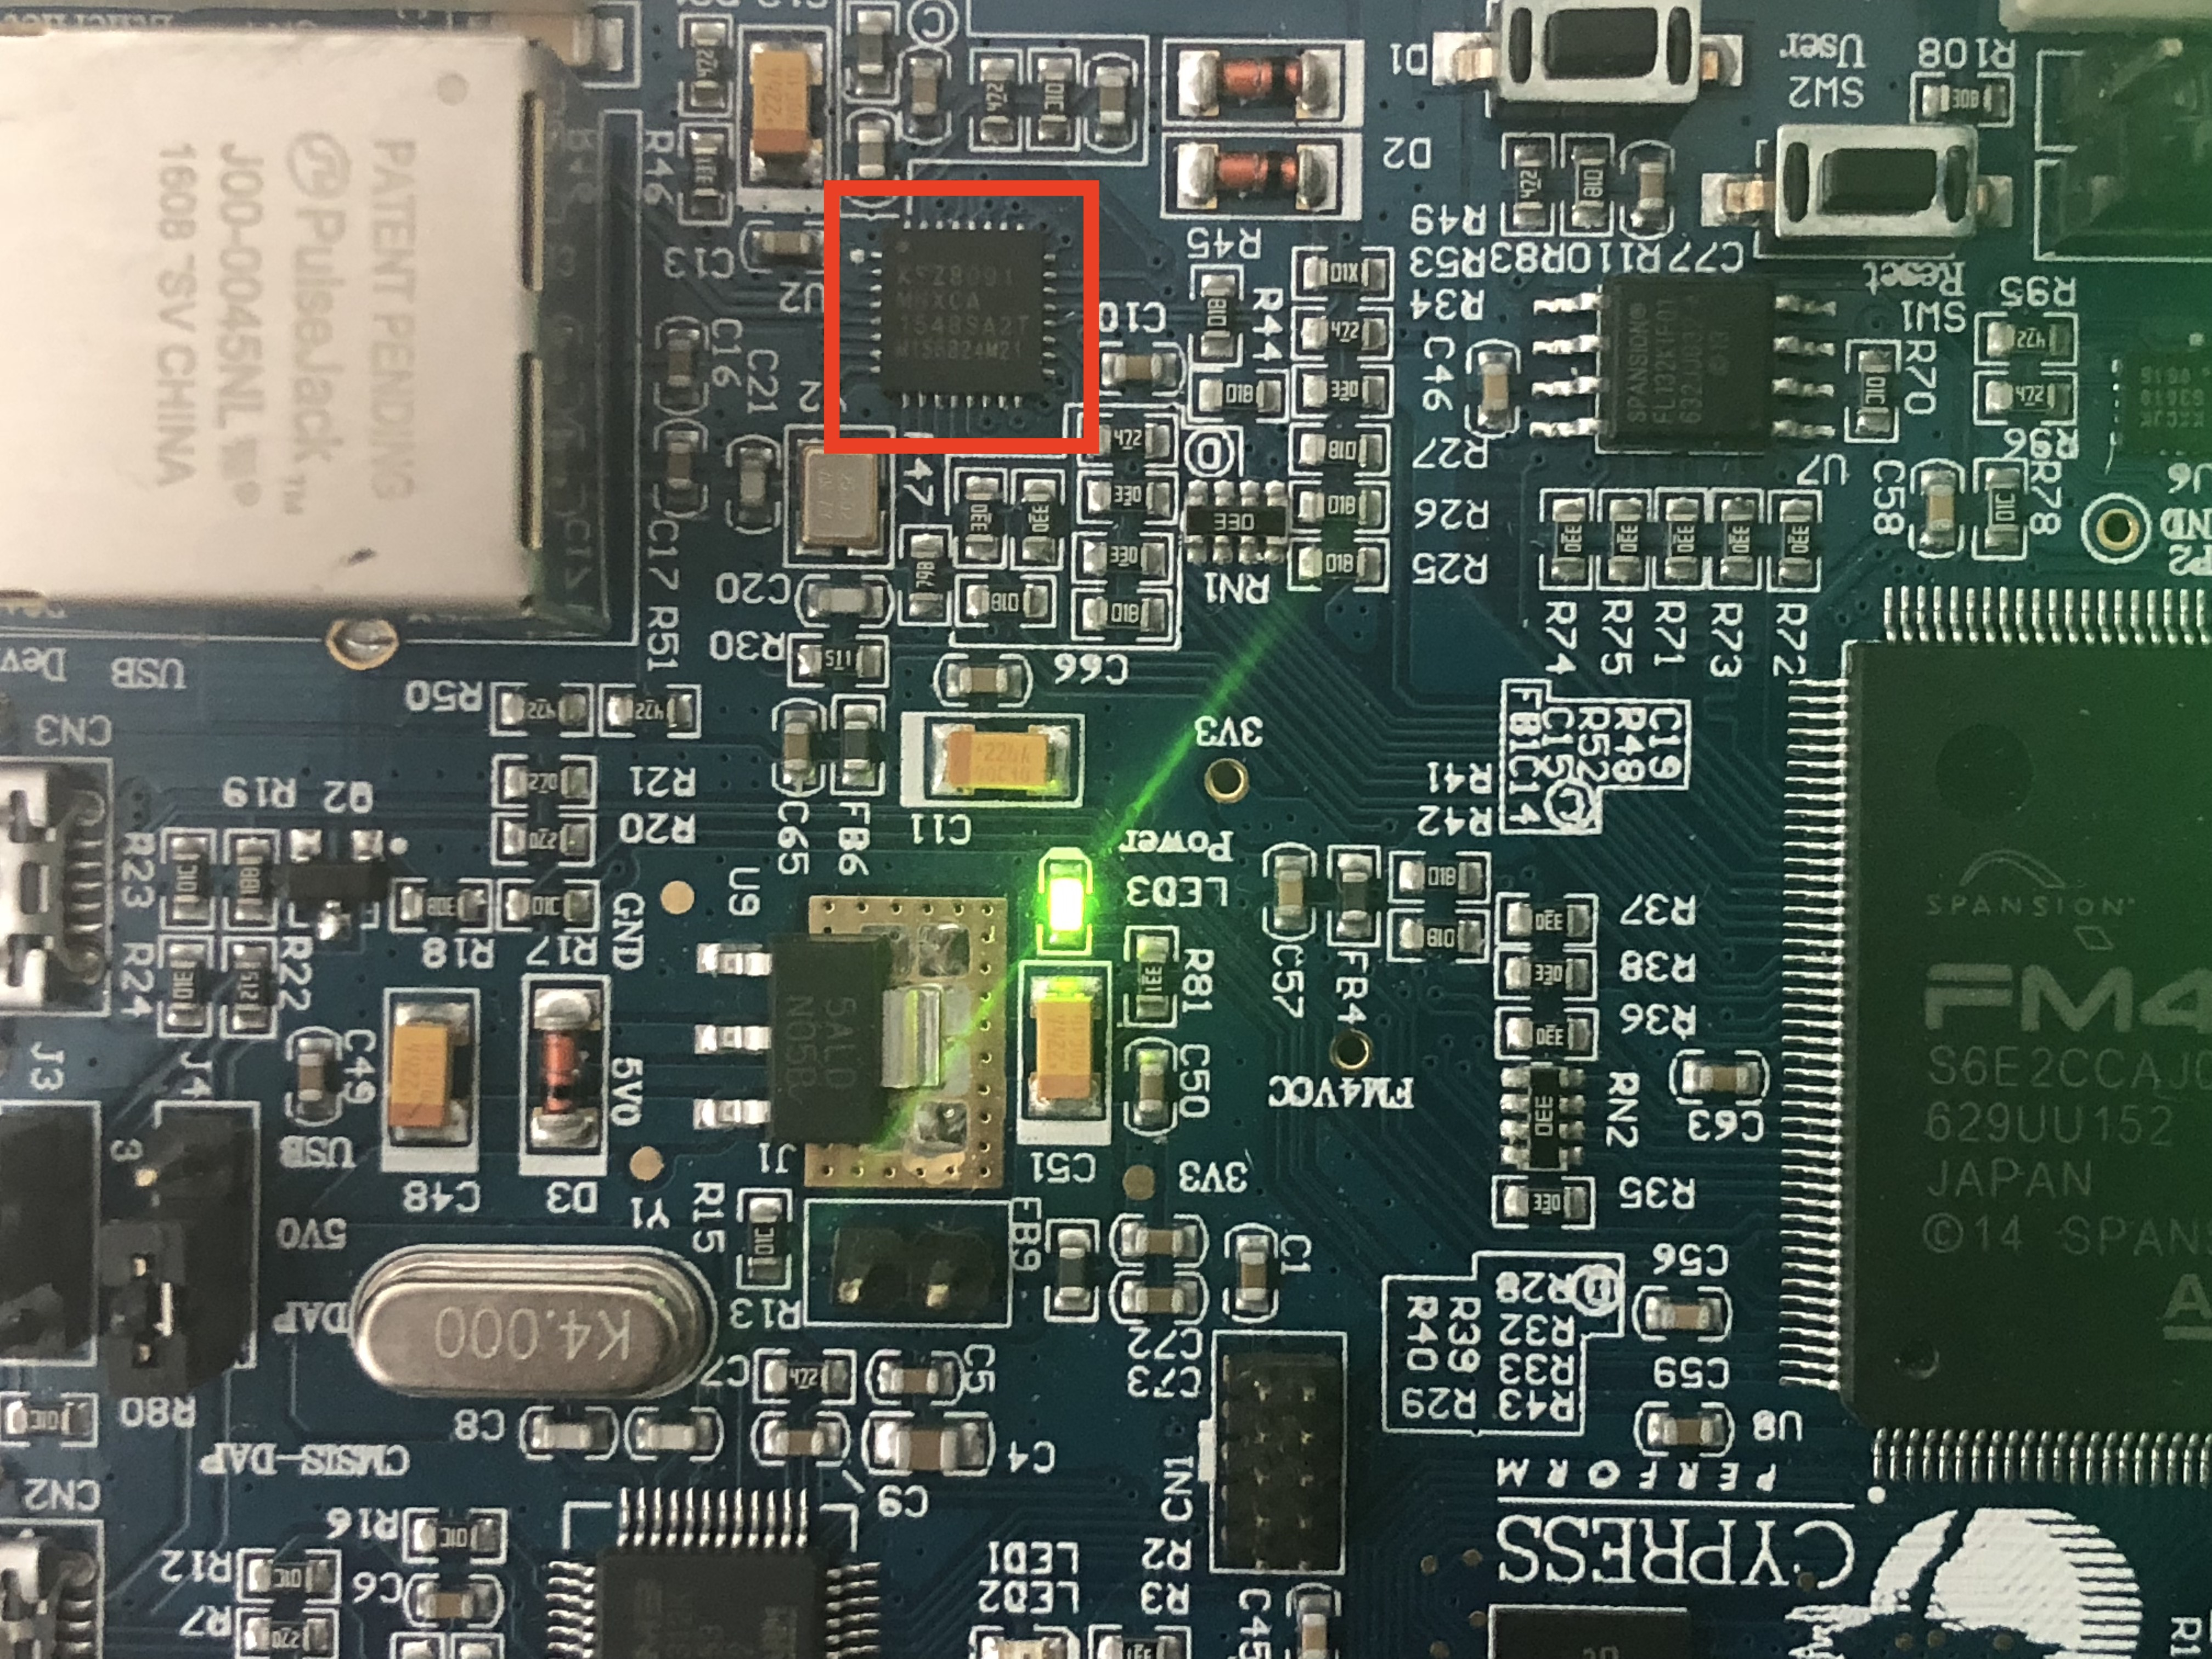
\includegraphics[width=0.4\textwidth]{./05_c/figures/kxcjk1013.png}
	\caption{Der Beschleunigungssensor des FM4-Boards (rot umrandet)}
	\label{fig:accelerometer}
\end{figure} 

In der Datei \filename{acceleration.c} (Gruppe \menuPath{src}) findest du eine Vorlage für diese Aufgabe.
In dieser fehlt noch die fertige Implementierung der Funktion \lstinline|cppp_rgbLEDAcceleration|.
Bei der Initialisierung des Boards wird eine Interrupt-Routine gestartet, sobald neue Messdaten des Beschleunigungssensor des Chips vorliegen.
Sofern die Routine ausgelöst wurde, wird die globale Variable \lstinline|cppp_accelerationDataAvailable| auf \lstinline|1| gesetzt.  
In dem Array \lstinline|float cppp_orientationValues[3]| werden die aktuellen X-,Y- und Z-Achsen-Orientierungen des Boards in alphabetischer Reihenfolge gespeichert. 
Gehe nun wie folgt vor:
%
\begin{enumerate}
	\item
    Gib auf dem Display kontinuierlich die aktuelle Orientierung des Boards aus.
    Setze hierzu den Cursor per \lstinline|setCursor| an die Position \lstinline|(0,319)| (linke obere Ecke des Displays) und gib die Daten in folgendem Format aus:
%	
	\cpppInputListing{05_c/listings/accelerometerLCDFormat.c}
%	
	\hints{
		\item Verwende zur Ausgabe von Variablen des Typs \lstinline|float| auf den Display die Funktion \lstinline|writeFloat| (im Header \filename{gfx.h}).
	}
%
	\item
    Nutze die Ergebnisse aus Teilaufgabe a um ein Schema zu erkennen, wann das Board sich nicht im Gleichgewicht befindet.
    Setze die RGB-LED auf Rot sofern sich das Board nicht im Gleichgewicht befindet und auf Grün falls ja.
    Gib ebenfalls auf dem Display aus, ob sich das Board im Gleichgewicht befindet (siehe Beispielformat in Teilaufgabe a). 
	\hints{
		\item Zum Ansteuern der RGB-LED kannst du in dieser Aufgabe als Vereinfachung den Header \lstinline|rgbled.h| (Gruppe: \menuPath{lib}) verwenden.
        Hierzu muss zunächst die Funktion \lstinline|cppp_initLEDs| einmalig aufgerufen werden.
        Beispielsweise kannst du mithilfe der Funktionen \lstinline|cppp_redLEDOn| und \lstinline|cppp_redLEDOff| die rote LED ein- bzw. ausschalten.
	}
\end{enumerate}

